\documentclass{beamer}

%\usepackage[utf8x]{inputenc}
\usepackage{graphicx}
\usepackage{hyperref}
\usepackage{xspace}
\usepackage{amsmath}
\usetheme{Madrid}

\definecolor{pink}{rgb}{1.0,.8,.8}
\definecolor{hotpink}{cmyk}{0.0,0.8,0,0.2}
\definecolor{softred}{rgb}{.9,.7,.7}
\definecolor{darkred}{rgb}{.8,.1,.1}
\definecolor{purple}{rgb}{.7,.0,.7}
\definecolor{darkgreen}{rgb}{.1,.45,.1}
\definecolor{lightblue}{rgb}{0.3,0.3,1.0}
\definecolor{grey}{rgb}{.5,.5,.5}


\newcommand{\darkred}[1]{\textcolor{darkred}{#1}}
\newcommand{\darkgreen}[1]{\textcolor{darkgreen}{#1}}
\newcommand{\hotpink}[1]{\textcolor{hotpink}{#1}}
\newcommand{\lightblue}[1]{\textcolor{lightblue}{#1}}
\newcommand{\blue}[1]{\textcolor{blue}{#1}}
\newcommand{\red}[1]{\textcolor{red}{#1}}
\newcommand{\green}[1]{\textcolor{green}{#1}}
\newcommand{\purple}[1]{\textcolor{purple}{#1}}
\newcommand{\grey}[1]{\textcolor{grey}{#1}}
\newcommand{\MetDeltaPhi}{\Delta\phi(\MET, \rm{lepton, jet})}
\newcommand{\MET}{\mbox{$E\kern-0.50em\raise0.10ex\hbox{/}_{T}$}}
\newcommand{\met}{\ensuremath{E_T^{miss}}\xspace}
\newcommand{\metrel}{\ensuremath{E_{T}^{miss,~\mathrm{Rel}}}\xspace} 
\newcommand{\tmet}{\ensuremath{E_{T}^{miss,~\mathrm{Track}}}\xspace} 
\newcommand{\ptll}{\ensuremath{p_{T}^{\ell\ell}}\xspace} 
\newcommand{\ptg}{\ensuremath{p_{T}^{\gamma}}\xspace} 
\newcommand{\ptZ}{\ensuremath{p_{T}^{Z}}\xspace} 
\newcommand{\METsig}{\MET_{\mathrm{sig}}}
\newcommand{\delPhiMet}{\min{\Delta\phi(\MET,l\mathrm{~or~jet}))}} 
\newcommand{\dphill}{\ensuremath{\Delta\phi_{\ell\ell}}} 
\newcommand{\SumEt}{\sum{E_{T}}}
\newcommand{\nunubar}{\nu \overline{\nu}}
\newcommand{\ttbar}{t \overline{t}}
\newcommand{\ppbar}{p \overline{p}}
\newcommand{\qqbar}{q \overline{q}}
\newcommand{\bbbar}{b \overline{b}}
\newcommand{\epem}{ e^+e^-}
\newcommand{\pt}{\ensuremath{p_{T}}\xspace}
\newcommand{\HWW}{H\rightarrow WW}
\newcommand{\BR}[1]{{\cal{B}} (#1)}
\newcommand{\zzllnunu}{\ensuremath{ZZ\to\ell\ell\nu\nu}\;}

\newcommand {\Dzero} {D\O\ }

\newcommand {\rmfrac}[2]{ $\frac{\mathrm{#1}}{\mathrm{#2}}$ }

\newcommand{\bc}{\begin{columns}}
\newcommand{\ec}{\end{columns}}
\newcommand{\fr}[2]{\begin{frame} \frametitle{#1} #2 \end{frame} }


\newcommand{\figbox}[5][]{
   \parbox{#2\textwidth}{
   \centering
   \includegraphics[#1,width=#3\textwidth]{#4}
   \ifthenelse{ \equal{}{#5} } {} {\\ #5}
}} 

\newcommand{\figboxv}[4]{
   \parbox{#1\textwidth}{
   \begin{center}
   \includegraphics[height=#2\textwidth]{#3}   
   \ifthenelse{ \equal{}{#4} } {} {
     \vspace{-0.35cm}
     \begin{center}
       #4
     \end{center}
   }
   \end{center}
}} 



\title[ WgamgamMCFilt ]
{ WgamgamMCFilt }

\author[Josh Kunkle]
  {Josh Kunkle}

\institute[UMD]{University of Maryland}

\date[March 10, 2014] % (optional)
{ 
  \vspace{0.5cm} \begin{center}\includegraphics[width=0.3\textwidth]{../UMDLogo.pdf}\end{center}
  \vspace{0.5cm}
}

\begin{document}

\maketitle

\fr{ The problem } {

    \scriptsize

    \begin{itemize}
        \item $W\gamma$ and $Z\gamma$ are the main backgrounds to the $W\gamma\gamma$ signal
        \item Despite the large sample size, a small number of events survive the full event selection
        \item This is particularly the case at large photon \pt, where we have the most signal sensitivity as well as TGC sensitivity
        \item Propose creating new samples with a \pt cut on the leading photon
    \end{itemize}

    \bc
        \column{0.5\textwidth}

        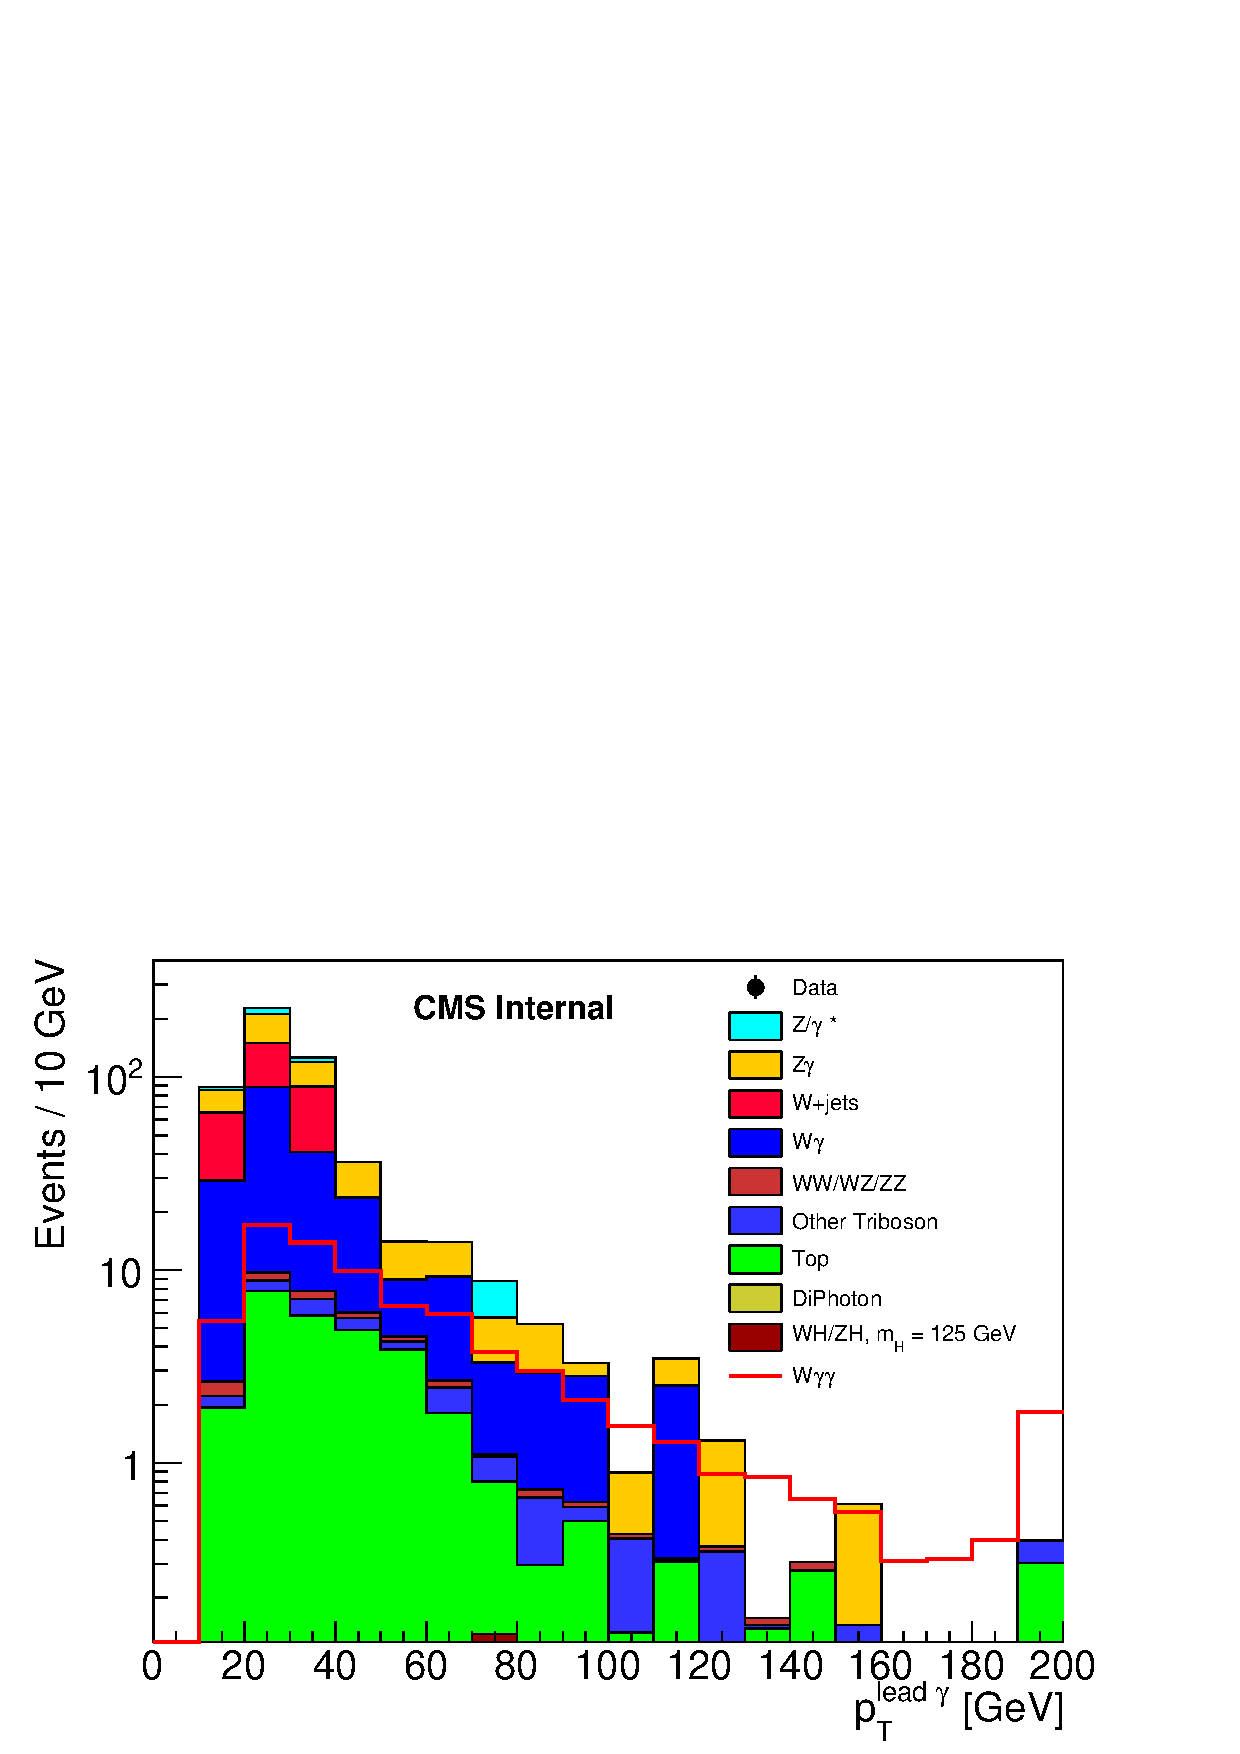
\includegraphics[width=0.8\textwidth]{Plots/ph_pt_mgg.pdf}

        \column{0.5\textwidth}

        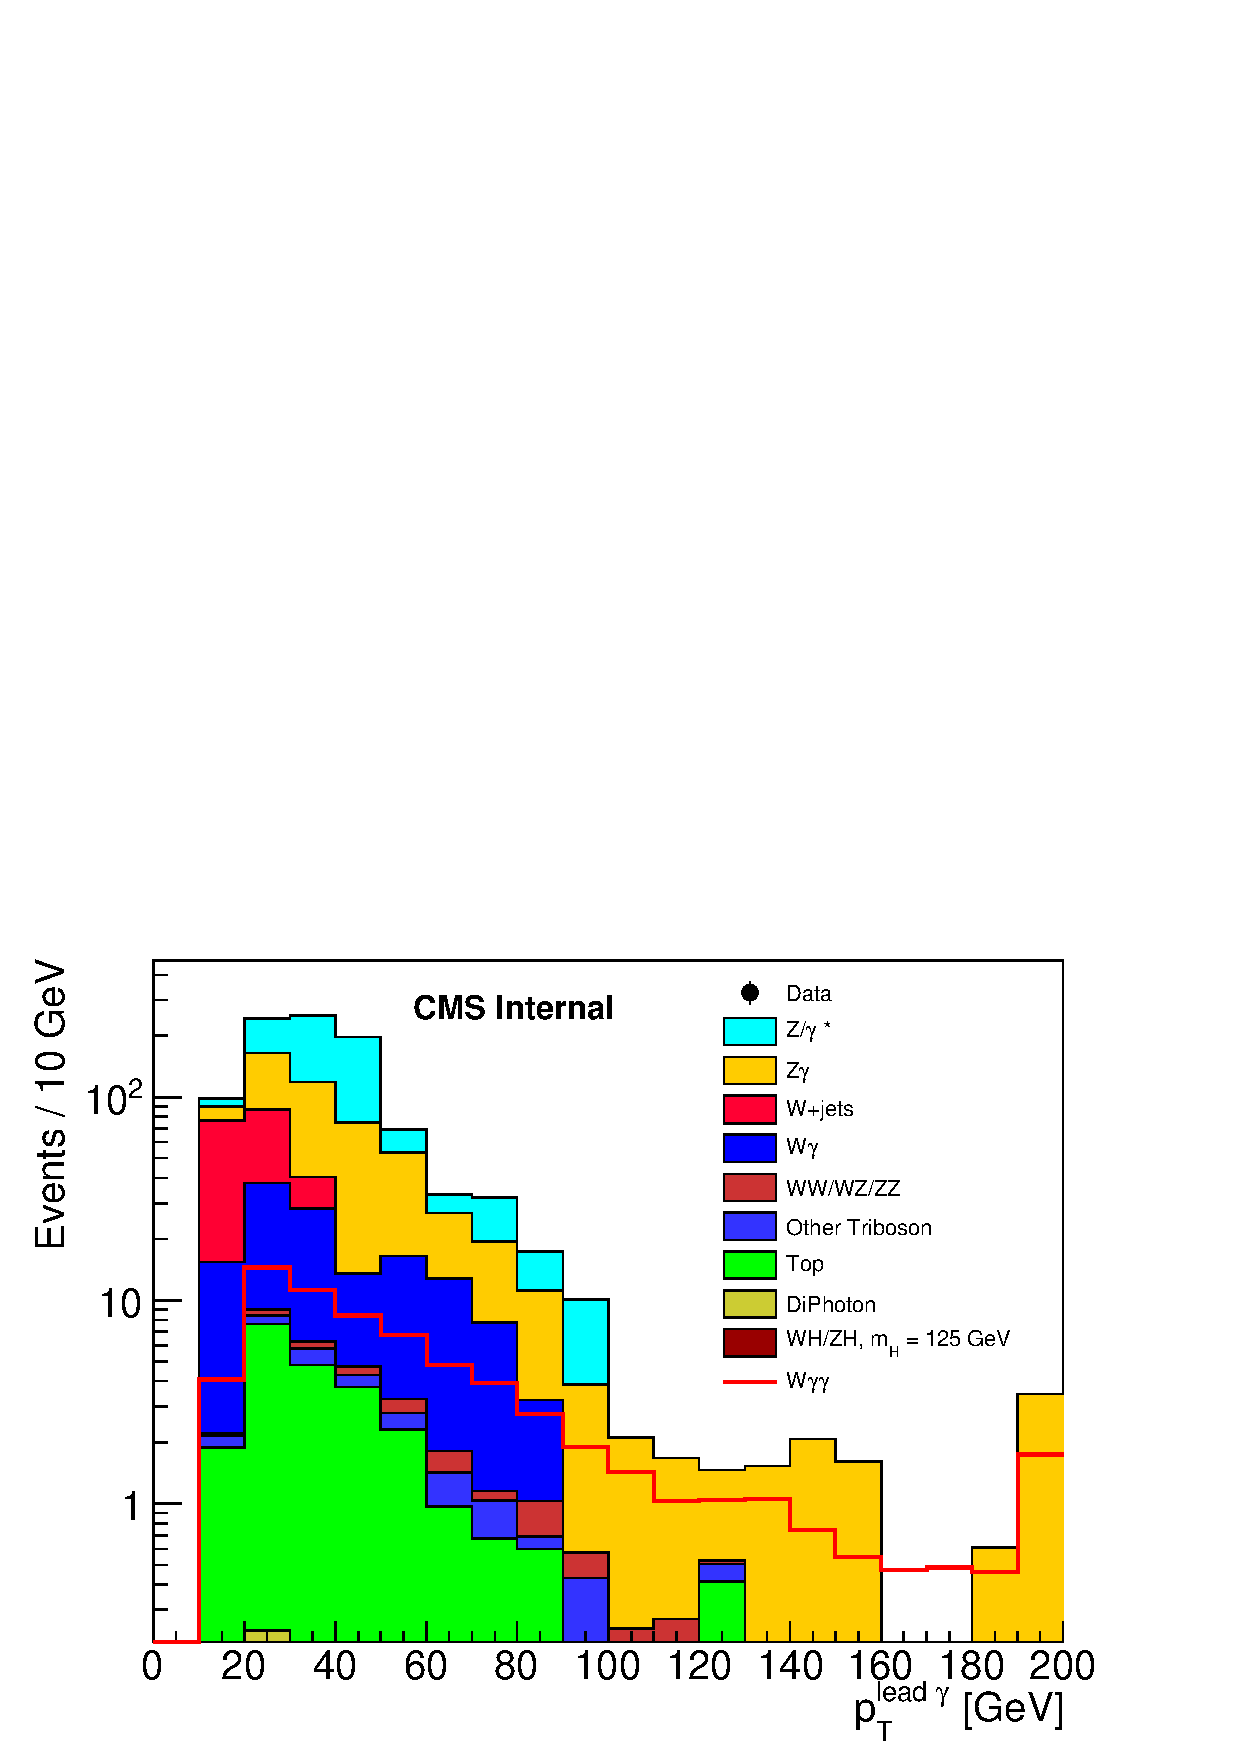
\includegraphics[width=0.8\textwidth]{Plots/ph_pt_egg.pdf}
    \ec


}

\fr{ Individual distributions } {

    \scriptsize
    \bc
        \column{0.5\textwidth}

        Muon Channel -- $W\gamma$

        \includegraphics[width=0.7\textwidth]{Plots/ph_pt_mgg_Wg.pdf}

        \column{0.5\textwidth}

        Electron Channel -- $W\gamma$

        \includegraphics[width=0.7\textwidth]{Plots/ph_pt_egg_Wg.pdf}

    \ec

    Muons
    \begin{tabular}{| l | c | c |}
       Lead photon \pt cut &  Backroung predition & stat uncertainty (\%) \\ \hline
        15 GeV  &  176   $\pm$ 19.7 & 11 \\ 
        40 GeV  &  37.5  $\pm$ 9.08 & 24  \\
        50 GeV  &  19.8  $\pm$ 6.61 & 33  \\
        60 GeV  &  15.4  $\pm$ 5.83 & 38  \\
    \end{tabular}

    Electrons
    \begin{tabular}{| l | c | c |}
       Lead photon \pt cut &  Backroung predition & stat uncertainty (\%) \\ \hline
        15 GeV  &  106   $\pm$ 15.3 & 14 \\ 
        40 GeV  &  41.9  $\pm$ 9.60 & 23  \\
        50 GeV  &  33.1  $\pm$ 8.53 & 26  \\
        60 GeV  &  19.8  $\pm$ 6.61 & 33  \\
    \end{tabular}

}

\fr{ Individual distributions } {

    \scriptsize
    \bc
        \column{0.5\textwidth}

        Muon Channel -- $Z\gamma$

        \includegraphics[width=0.7\textwidth]{Plots/ph_pt_mgg_Zg.pdf}

        \column{0.5\textwidth}

        Electron Channel -- $Z\gamma$

        \includegraphics[width=0.7\textwidth]{Plots/ph_pt_egg_Zg.pdf}
    \ec

    Muons
    \begin{tabular}{| l | c | c |}
       Lead photon \pt cut &  Backroung predition & stat uncertainty (\%) \\ \hline
        15 GeV  &  142   $\pm$ 8.2 & 5.8  \\ 
        40 GeV  &  30.5  $\pm$ 3.78 & 12  \\
        50 GeV  &  17.8  $\pm$ 2.89 & 16  \\
        60 GeV  &  12.7  $\pm$ 2.43 & 19  \\
    \end{tabular}

    Electrons
    \begin{tabular}{| l | c | c |}
       Lead photon \pt cut &  Backroung predition & stat uncertainty (\%) \\ \hline
        15 GeV  &  318   $\pm$ 12.2 & 3.8 \\ 
        40 GeV  &  148   $\pm$ 8.34 & 5.6  \\
        50 GeV  &  86.7  $\pm$ 6.37 & 7.3  \\
        60 GeV  &  49.7  $\pm$ 6.61  & 13  \\
    \end{tabular}


}

%Muons
%
%No cut
%Zgamma :         142.441285 +- 8.169568
%Inclusive W :    146.260445 +- 42.221753
%Wgamma :         176.267663 +- 19.707324
%
%pt 40
%Zgamma :         30.456195 +- 3.777626
%Inclusive W :    0.000000 +- 0.000000
%Wgamma :         37.456878 +- 9.084627
%
%
%pt 50
%Zgamma :         17.805160 +- 2.888378
%Inclusive W :    0.000000 +- 0.000000
%Wgamma :         19.830112 +- 6.610037
%
%pt 60
%Zgamma :         12.651035 +- 2.434693
%Inclusive W :    0.000000 +- 0.000000
%Wgamma :         15.423420 +- 5.829505
%
%Electrons
%
%No cut
%Zgamma :         317.681550 +- 12.200486
%Inclusive W :    121.883706 +- 38.543011
%Wgamma :         105.760599 +- 15.265228
%
%
%pt 40
%Zgamma :         148.532524 +- 8.342418
%Inclusive W :    0.000000 +- 0.000000
%Wgamma :         41.863570 +- 9.604162
%
%pt 50
%Zgamma :         86.683018 +- 6.373062
%Inclusive W :    0.000000 +- 0.000000
%Wgamma :         33.050187 +- 8.533522
%
%pt 60
%Zgamma :         49.667026 +- 4.824088
%Inclusive W :    0.000000 +- 0.000000
%Wgamma :         19.830112 +- 6.610037

\end{document}


